\documentclass[a4paper,12pt]{article}
\usepackage[left=2.5cm,right=2.5cm,top=2.5cm,bottom=2.5cm]{geometry} % Adjust page margins
\usepackage{xcolor,graphicx,framed}
\usepackage[normalem]{ulem}
\usepackage{amsmath}
\usepackage{cases}
\usepackage{gensymb}
\usepackage{chemmacros}
\setlength{\extrarowheight}{0.35cm}
%\usepackage{lastpage} % Required to print the total number of pages

\begin{document}

\newcommand{\HRule}{\rule{\linewidth}{0.4mm}} % Defines a new command for the horizontal lines, change thickness here

%----------------------------------------------------------------------------------------
%	HEADING SECTIONS
%----------------------------------------------------------------------------------------

\begin{minipage}{0.7\textwidth}
\begin{flushleft} 
\textsc{Universidad del Valle de Guatemala \\
Campus Central \\
Facultad de Ciencias y Humanidades \\
Departamento de Qu\'imica \\
Segundo ciclo, 2014 \\
Fisicoqu\'imica 1 \\
}
\end{flushleft}
\end{minipage}
~
\begin{minipage}{0.2\textwidth}
\begin{flushright}

\includegraphics[scale=0.3]{Logo_UVG} % Include a department/university logo
\end{flushright}
\end{minipage}\\

%----------------------------------------------------------------------------------------
%	TITLE SECTION
%----------------------------------------------------------------------------------------

\begin{center}
\HRule \\[0.4cm]
{ \bfseries Soluciones propuestas a los ejercicios en clase, 5}\\ % Title of your document
\HRule \\[0.4cm]
\end{center}

%----------------------------------------------------------------------------------------

\begin{enumerate}

 \item \textbf{\textit{(McQuarrie 19-37)} Las entalp\'ias molares estandar de combusti\'on para los is\'omeros $m\mbox{-xileno}$ y $p\mbox{-xileno}$ son $-4553.9\;\mbox{kJ}\cdot\mbox{mol}^{-1}$ y $-4556.8\;\mbox{kJ}\cdot\mbox{mol}^{-1}$, respectivamente. Usar estos datos, junto con la ley de Hess, para calcular el valor de $\Delta_rH^\standardstate$ para la reacci\'on:}
$$m\mbox{-xileno}\rightarrow p\mbox{-xileno}$$ % Problema 5-37

La informaci\'on que nos dan son entalp\'ias molares est\'andar de combusti\'on, por lo que no podemos hacer el mismo procedimiento que hacemos con las entalp\'ias de formaci\'on para determinar $\Delta_rH^\standardstate$. Pero usando la ley de Hess podemos utilizar la informaci\'on que nos dan. Para hacer eso, es conveniente escribir expl\'icitamente las reacciones involucradas. Como son is\'omeros, el $m\mbox{-xileno}$ y $p\mbox{-xileno}$ tienen la misma f\'ormula, $\mbox{C}_8\mbox{H}_{10}$, y la reacci\'on de combusti\'on es:
$$\mbox{C}_8\mbox{H}_{10}+\frac{21}{2}\,\mbox{O}_2\;\rightarrow\; 8\,\mbox{CO}_2+5\,\mbox{H}_2\mbox{O}$$
Al invertir la reacci\'on del $p\mbox{-xileno}$ y sumarla con la del $m\mbox{-xileno}$, obtendr\'iamos la reacci\'on que nos interesa, por lo que podemos sumar las entalp\'ias molares est\'andar de combusti\'on, tomando en cuenta que la del $p\mbox{-xileno}$ se le cambia de signo al invertir la reacci\'on:
\begin{center}
\begin{tabular}{c c | c}
& \quad & $\Delta H^\standardstate$ \\
$\underbrace{\mbox{C}_8\mbox{H}_{10}}_\text{m\mbox{-xileno}}+\frac{21}{2}\,\mbox{O}_2\;\rightarrow\; 8\,\mbox{CO}_2+5\,\mbox{H}_2\mbox{O}$ & \quad & $-4553.9\;\mbox{kJ}\cdot\mbox{mol}^{-1}$ \\
$8\,\mbox{CO}_2+5\,\mbox{H}_2\mbox{O}\;\rightarrow\;\underbrace{\mbox{C}_8\mbox{H}_{10}}_\text{p\mbox{-xileno}}+\frac{21}{2}\,\mbox{O}_2$ & \quad & $+4556.8\;\mbox{kJ}\cdot\mbox{mol}^{-1}$ \\ \hline
$m\mbox{-xileno}\rightarrow p\mbox{-xileno}$ & \quad & $+2.9\;\mbox{kJ}\cdot\mbox{mol}^{-1}$
\end{tabular}
\end{center}

As\'i que $\Delta_rH^\standardstate=+2.9\;\mbox{kJ}\cdot\mbox{mol}^{-1}$ para la reacci\'on dada.

\newpage

 \item \textbf{\textit{(McQuarrie 19-42)} Usar los siguientes datos para calcular el valor de $\Delta_{vap}H^\standardstate$ del agua a $298\;\mbox{K}$: $\Delta_{vap}H^\standardstate\mbox{ a 373 K}=40.7\;\mbox{kJ}\cdot\mbox{mol}^{-1}$; $\bar{C}_P\mbox{(l)}=75.2\;\mbox{J}\cdot\mbox{mol}^{-1}\cdot\mbox{K}^{-1}$; $\bar{C}_P\mbox{(g)}=33.6\;\mbox{J}\cdot\mbox{mol}^{-1}\cdot\mbox{K}^{-1}$. Comparar el resultado con valor que se obtendr\'ia a partir de $\Delta_{f}H^\standardstate=-285.83\;\mbox{kJ}\cdot\mbox{mol}^{-1}$ para $\mbox{H}_2\mbox{O(l)}$ y $\Delta_{f}H^\standardstate=-241.8\;\mbox{kJ}\cdot\mbox{mol}^{-1}$ para $\mbox{H}_2\mbox{O(g)}$, a $25\celsius$.} % Problema 5-42

Si observamos el siguiente ciclo, podemos deducir la relaci\'on entre las entalp\'ias a las dos temperaturas (lo que es equivalente a aplicar la ley de Kirchhoff directamente):

\begin{center}
\begin{tabular}{r c c c l c | c}
& & & & & \quad & T \\\hline
& $\mbox{H}_2\mbox{O(l)}$ & $\xrightarrow{\Delta_{vap}H^\standardstate}$ & $\mbox{H}_2\mbox{O(g)}$ & & \quad\quad & $298\;\mbox{K}$ \\
 ${\bar{C}_P\mbox{(l)}}$ & $\downarrow$ & & $\uparrow$ & ${\bar{C}_P\mbox{(g)}}$ & \quad\quad & \\
& $\mbox{H}_2\mbox{O(l)}$ & $\xrightarrow{\Delta_{vap}H^\standardstate}$ & $\mbox{H}_2\mbox{O(g)}$ & & \quad\quad & $373\;\mbox{K}$ \\\hline
\end{tabular}
\end{center}

Con lo que obtenemos que:

\begin{tabular}{r c l}
$\Delta_{vap}H^\standardstate(298\;\mbox{K})$ & $=$ & $\int_{298}^{373}C_P\mbox{(l)}dT+\Delta_{vap}H^\standardstate(373\;\mbox{K})+\int_{373}^{298}C_P\mbox{(g)}dT$ \\
& $=$ & $-\int_{373}^{298}C_P\mbox{(l)}dT+\Delta_{vap}H^\standardstate(373\;\mbox{K})+\int_{373}^{298}C_P\mbox{(g)}dT$ \\
& $=$ & $\Delta_{vap}H^\standardstate(373\;\mbox{K})+\int_{373}^{298}\left[C_P\mbox{(g)}-C_P\mbox{(l)}\right]dT$ 
\end{tabular}

(Que es la ley de Kirchhoff.) Si dividimos todos los terminos por $n$, podemos trabajar con cantidades molares:

\begin{tabular}{r c l}
$\Delta_{vap}\bar{H}^\standardstate(298\;\mbox{K})$ & $=$ & $\Delta_{vap}\bar{H}^\standardstate(373\;\mbox{K})+\int_{373}^{298}\left[\bar{C}_P\mbox{(g)}-\bar{C}_P\mbox{(l)}\right]dT$ \\
& $=$ & $\Delta_{vap}\bar{H}^\standardstate(373\;\mbox{K})+\left[\bar{C}_P\mbox{(g)}-\bar{C}_P\mbox{(l)}\right](298\;\mbox{K}-373\;\mbox{K})$ \\
& $=$ & $40.7\times 10^3\;\mbox{J}\cdot\mbox{mol}^{-1}+$ \\
& & $\left(33.6\;\mbox{J}\cdot\mbox{K}^{-1}\cdot\mbox{mol}^{-1}-75.2\;\mbox{J}\cdot\mbox{K}^{-1}\cdot\mbox{mol}^{-1}\right)(298\;\mbox{K}-373\;\mbox{K})$ \\
& $=$ & $43.8\;\mbox{kJ}\cdot\mbox{mol}^{-1}$
\end{tabular}

Por otra parte, podemos usar los valores de entalp\'ias de formaci\'on para determinar $\Delta_r\bar{H}^\standardstate$ de la reacci\'on de vaporizaci\'on (en otras palabras, determinar $\Delta_{vap}\bar{H}^\standardstate$ a $25\celsius$):
$$\mbox{H}_2\mbox{O(l)}\;\xrightarrow{\Delta_{vap}H^\standardstate}\;\mbox{H}_2\mbox{O(g)}$$
de la siguiente manera:
\begin{center}
\begin{tabular}{c c l}
$\Delta_{r} H^\standardstate$ & $=$ & $\sum_{Productos}\nu \Delta_{f}H^\standardstate-\sum_{Reactivos}\nu\Delta_{f}H^\standardstate$ \\
$\Delta_{vap}\bar{H}^\standardstate$ & $=$ & $\Delta_{f}H^\standardstate[\mbox{H}_2\mbox{O(g)}]-\Delta_{f}H^\standardstate[\mbox{H}_2\mbox{O(l)}]$ \\
& $=$ & $-241.8\;\mbox{kJ}\cdot\mbox{mol}^{-1}-(-285.83\;\mbox{kJ}\cdot\mbox{mol}^{-1})$ \\
& $=$ & $44.0\;\mbox{kJ}\cdot\mbox{mol}^{-1}$
\end{tabular}
\end{center}

 \item \textbf{\textit{(McQuarrie 19-22)} Un mol de etano a $25\celsius$ y una atm\'osfera es calentado hasta $1200\celsius$ a presi\'on constante. Asumiendo un comportamiento ideal, calcular los valores de $w$, $q$, $\Delta U$ y $\Delta H$ si su capacidad calor\'ifica molar est\'a dada por:
$$\bar{C}_P/R=0.06436+(2.137\times 10^{-2}\;\mbox{K}^{-1})T-(8.263\times 10^{-6}\;\mbox{K}^{-2})T^2+(1.024\times 10^{-9}\;\mbox{K}^{-3})T^3$$
para el rango de temperatura dado. Repetir el c\'alculo para un proceso a volumen constante.} %Problema 5-22

Ya sea calentamiento (de $T_1=25\celsius+273.15=298.15\;\mbox{K}$ a $T_2=1200\celsius+273.15=1473.15\;\mbox{K}$) a presi\'on constante o a volumen constante, asumiendo un comportamiento ideal tendr\'iamos que $\Delta H=\int_{T_1}^{T_2}C_PdT$, tomando $C_P=n\bar{C}_P$ con $n=1\;\mbox{mol}$, y $\Delta U=\int_{T_1}^{T_2}C_VdT$, teniendo $C_P-C_V=nR$ \'o $C_V=C_P-nR$, as\'i que:

\begin{tabular}{r c l}
$\Delta H$ & $=$ & $(1\;\mbox{mol})R\int_{298.15}^{1473.15}[0.06436+(2.137\times 10^{-2}\;\mbox{K}^{-1})T-(8.263\times 10^{-6}\;\mbox{K}^{-2})T^2$ \\
& & $\quad+(1.024\times 10^{-9}\;\mbox{K}^{-3})T^3]dT$ \\
& $=$ & $(1\;\mbox{mol})R\left[0.06436\times T+\left(2.137\times 10^{-2}\;\mbox{K}^{-1}\right)\frac{T^2}{2}-\left(8.263\times 10^{-6}\;\mbox{K}^{-2}\right)\frac{T^3}{3}\right.$ \\
& & $\quad+\left.\left.\left(1.024\times 10^{-9}\;\mbox{K}^{-3}\right)\frac{T^4}{4}\right]\right|_{298.15}^{1473.15}$ \\
& $=$ & $(14785.15\;\mbox{K}\cdot\mbox{mol})(8.314\;\mbox{J}\cdot\mbox{K}^{-1}\cdot\mbox{mol}^{-1})=122.9\;\mbox{kJ}$
\end{tabular}

Y:

\begin{tabular}{r c l}
$\Delta U$ & $=$ & $\int_{298.15}^{1473.15}C_VdT=\int_{298.15}^{1473.15}(C_P-nR)dT$ \\
& $=$ & $\int_{298.15}^{1473.15}C_PdT-nR\int_{298.15}^{1473.15}dT$ \\
& $=$ & $14785.15\;\mbox{K}\cdot\mbox{mol}\times R-(1\;\mbox{mol})\times R\times(1473.15\;\mbox{K}-298.15\;\mbox{K})$ \\
& $=$ & $(13610.15\;\mbox{K}\cdot\mbox{mol})(8.314\;\mbox{J}\cdot\mbox{K}^{-1}\cdot\mbox{mol}^{-1})=113.2\;\mbox{kJ}$
\end{tabular} 

Para el caso del calentamiento a presi\'on constante, tenemos que $q=q_P=\Delta H=122.9\;\mbox{kJ}$ y $w=\Delta U-q=113.2\;\mbox{kJ}-122.9\;\mbox{kJ}=-9.77\;\mbox{kJ}$. En cambio, para el calentamiento a volumen constante, tenemos que $q=q_V=\Delta U=113.2\;\mbox{kJ}$ y $w=\Delta U-q=0$.

 \item \textbf{\textit{(McQuarrie 19-34)} Dados los siguientes datos del sodio, graficar $\bar{H}(T)-\bar{H}(0)$ en funci\'on de $T$ para el sodio: punto de fusi\'on, $361\;\mbox{K}$; punto de ebullici\'on, $1156\;\mbox{K}$; $\Delta_{fus}H^\standardstate=2.60\;\mbox{kJ}\cdot\mbox{mol}^{-1}$; $\Delta_{vap}H^\standardstate=97.4\;\mbox{kJ}\cdot\mbox{mol}^{-1}$; $\bar{C}_P(s)=28.2\;\mbox{J}\cdot\mbox{mol}^{-1}\cdot\mbox{K}^{-1}$; $\bar{C}_P\mbox{(l)}=32.7\;\mbox{J}\cdot\mbox{mol}^{-1}\cdot\mbox{K}^{-1}$; $\bar{C}_P\mbox{(g)}=20.8\;\mbox{J}\cdot\mbox{mol}^{-1}\cdot\mbox{K}^{-1}$.} % Problema 5-34

Para calcular el valor de $\bar{H}(T)-\bar{H}(0)$ con la informaci\'on dada, recordemos que cuando hay cambio de temperatura sin cambio de fase, el cambio de entalp\'ia se calcula como $\Delta H=\int_{T_1}^{T_2}C_PdT$, y cuando hay cambio de fase, habr\'ia un salto dado por el valor de $\Delta_{trs} H$. As\'i que para temperaturas menores al punto de fusi\'on (tomando en cuenta que las capacidades calor\'ificas dadas son constantes), tendr\'iamos:
$$\bar{H}(T)-\bar{H}(0)=\int_{0}^{T}\bar{C}_P\mbox{(s)}dT=\bar{C}_P\mbox{(s)}\times T$$
Para temperaturas entre el punto de fusi\'on y el punto de ebullici\'on:

\begin{tabular}{r c l}
$\bar{H}(T)-\bar{H}(0)$ & $=$ & $\int_{0}^{361}\bar{C}_P\mbox{(s)}dT+\Delta_{fus}\bar{H}^\standardstate+\int_{361}^{T}\bar{C}_P\mbox{(l)}dT$ \\
& $=$ & $\bar{C}_P\mbox{(s)}\times 361\;\mbox{K}+\Delta_{fus}\bar{H}^\standardstate+\bar{C}_P\mbox{(l)}(T-361\;\mbox{K})$
\end{tabular}

Y para temperaturas m\'as altas que el punto de ebullici\'on:

\begin{tabular}{r c l}
$\bar{H}(T)-\bar{H}(0)$ & $=$ & $\int_{0}^{361}\bar{C}_P\mbox{(s)}dT+\Delta_{fus}\bar{H}^\standardstate+\int_{361}^{1156}\bar{C}_P\mbox{(l)}dT+\Delta_{vap}\bar{H}^\standardstate+$ \\
& & $\quad\int_{1156}^{T}\bar{C}_P\mbox{(g)}dT$ \\
& $=$ & $\bar{C}_P\mbox{(s)}\times 361\;\mbox{K}+\Delta_{fus}\bar{H}^\standardstate+\bar{C}_P\mbox{(l)}(1156\;\mbox{K}-361\;\mbox{K})+$ \\
& & $\quad\Delta_{vap}\bar{H}^\standardstate+\bar{C}_P\mbox{(g)}(T-1156\;\mbox{K})$
\end{tabular}

Es decir:
\[
 \bar{H}(T)-\bar{H}(0) =
  \begin{cases}
  28.2\;\mbox{J}\cdot\mbox{K}^{-1} (T) & \text{si }\;\;\; 0 \leq T < 361 \\
  12.7802\;\mbox{kJ}+32.7\;\mbox{J}\cdot\mbox{K}^{-1} (T-361\;\mbox{K})  & \text{si }\; 361 \leq T < 1156 \\
  136.1767\;\mbox{kJ}+20.8\;\mbox{J}\cdot\mbox{K}^{-1} (T-1156\;\mbox{K}) & \text{si }\;\;\;\;\; T \geq 1156
  \end{cases}
\]

Que gr\'aficamente se ver\'ia de la siguiente manera:
\begin{center}
 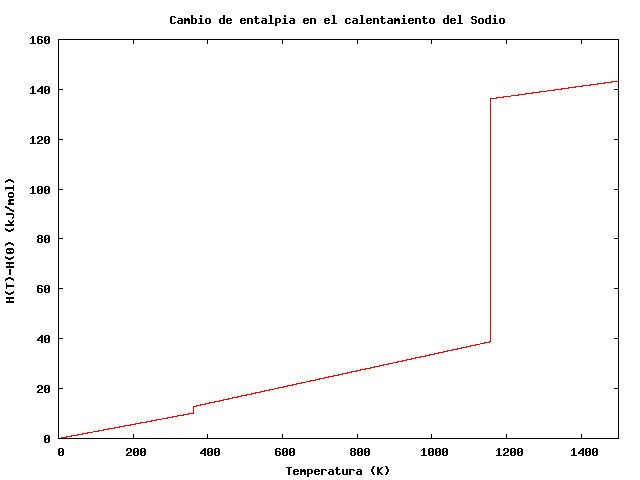
\includegraphics[scale=0.9]{figure3}
\end{center}

 \item \textbf{\textit{(McQuarrie 19-29)} A partir de $H=U+PV$, mostrar que:
$$\left(\frac{\partial U}{\partial T}\right)_P=C_P-P\left(\frac{\partial V}{\partial T}\right)_P$$
Interpretar f\'isicamente este resultado.} % Problema 5-29

Si sacamos la derivada parcial con respecto a $T$ a $P$ constante para ambos lados de $H=U+PV$, tendr\'iamos:
$$\left(\frac{\partial H}{\partial T}\right)_P=\left(\frac{\partial }{\partial T}\right)_P(U+PV)=\left(\frac{\partial U}{\partial T}\right)_P+P\left(\frac{\partial V}{\partial T}\right)_P$$
Identificando que $(\partial H/\partial T)_P=C_P$ y reordenando, se obtiene:
$$\left(\frac{\partial U}{\partial T}\right)_P=C_P-P\left(\frac{\partial V}{\partial T}\right)_P$$

Lo que indicar\'ia que conforme vamos calentando una sustancia (una forma de cambiarle la temperatura), la cantidad de energ\'ia interna no aumenta directamente proporcional a la capacidad calor\'ifica (en cuyo caso todo el calor se transformar\'ia a energ\'ia interna), sino que hay que contrarrestar el cambio de volumen que tendr\'ia la sustancia con el cambio de temperatura.

\end{enumerate}
 
\end{document}
